\section{Reference model and results}
\begin{frame}{Outline}
	\tableofcontents[currentsection]
\end{frame}


\subsection{Creating a spherical sample}
\begin{frame}{Creating a spherical sample}
\begin{columns}
	\begin{column}{0.75\textwidth}
		\begin{itemize}[<+->]
			\item Sample usually cuboid with periodic boundary conditions (PBC)
			\item What we want: Sphere under influence of gravity
			\item Strategy:
			\begin{enumerate}
				\item Equilibration and heating of an arbitrary cuboid sample
				\item Cut out sphere (spacing!) + ground
				\item Make the ground fixed
				\item Continue equilibration under influence of gravity
			\end{enumerate}
			\vspace{1cm}
			\item Diameter $\sim \SI{400}{\angstrom}$ vs. a few \si{\micro\meter} in reality
			\item Motivated by work of \cite{glosli2007extending}
		\end{itemize}
	\end{column}
	\begin{column}{0.25\textwidth}
		\vspace{-1.35\baselineskip}
		\visible<8->{
		\begin{figure}
			\centering
			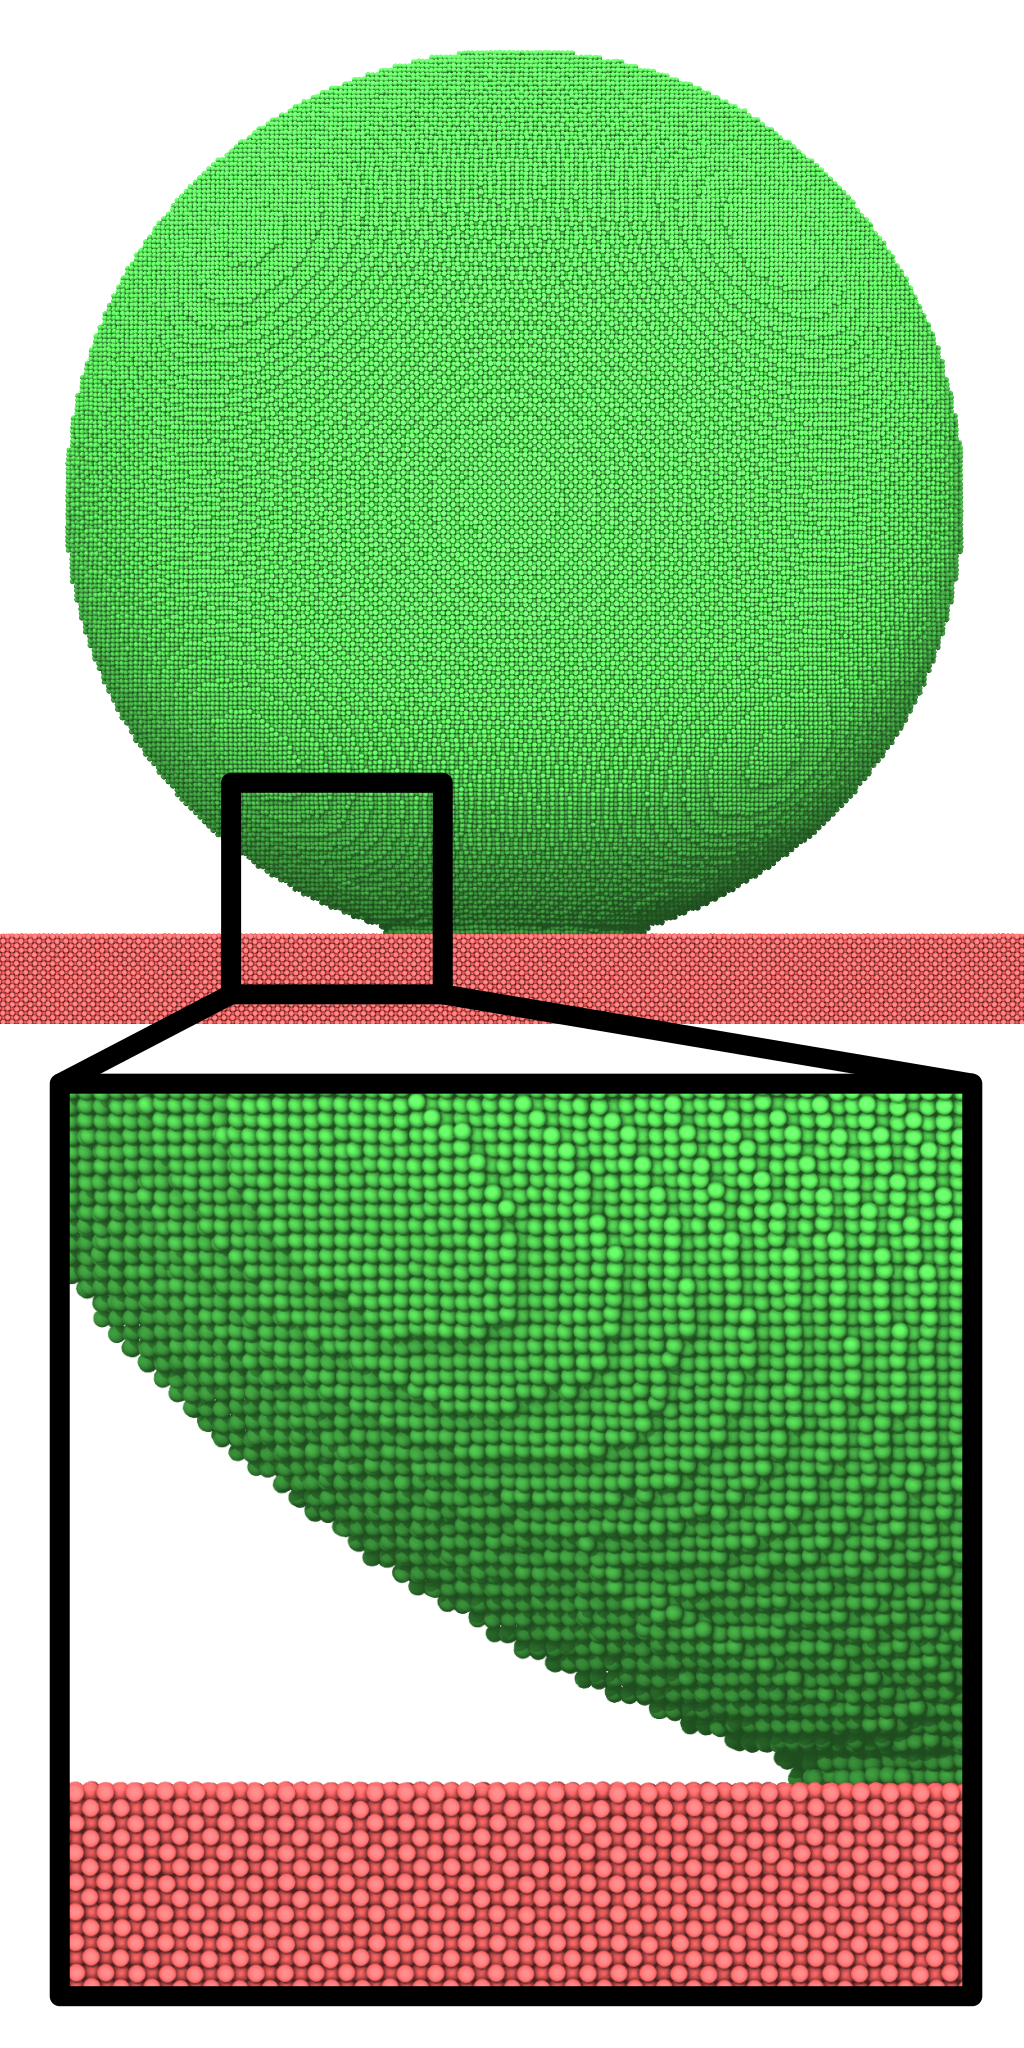
\includegraphics[width=0.85\textwidth]{single/img/equilibration/sphere_zoom_vertical.png}
			\vspace{-0.6\baselineskip}
			\caption{Fully equilibrated aluminium sphere (green) on ground (red).}
		\end{figure}
		}
	\end{column}
\end{columns}
\end{frame}


\subsection{Influence of the laser's power}
\begin{frame}{Influence of the laser's power}
	\begin{itemize}
		\item Approximations make it hard to map simulation data to
	\end{itemize}
\end{frame}


\subsection{Cutting the scanning speed in half}
\begin{frame}{Cutting the scanning speed in half}
	\missing
\end{frame}
